\chapter{Temporal Coherence and First-Order (Amplitude) Interferometry}
\label{chap:e09}

\begin{chapteropening}
By now we know that light is the excitation of a set of modes, whose positive-frequency field operator \(\hat E^{(+)}\) was introduced in Chapter \ref{chap:e05}; and that a detector counts only intensity and cannot see the phase of the field is exactly what the photodetection of Chapter \ref{chap:e07} taught us (one optical cycle is only a few femtoseconds, so any detector is far too "slow," and can only average away the oscillation and leave the energy). We also know that a beam of light "remembers its own phase" only for a coherence time \(\tau_c\simeq1/\Delta\nu\) (Chapter \ref{chap:e02}). But if the phase cannot be seen, on what grounds do we speak of "coherence"? The answer is interference: split a beam into two paths, send them along different optical paths, and recombine them, and the phase difference will show itself in the \emph{intensity}: bright fringes, dark fringes, one after another. What this chapter does is bring the abstract first-order degree of coherence \(g^{(1)}(\tau)\) down to a tangible interferometer you can see and touch: we derive the fringe-intensity formula, define the fringe visibility, and prove that "the visibility is the direct reading of how much phase the field still remembers"; then, following the Wiener--Khinchin theorem, we build a bridge explaining why "how fast the fringes fade with optical-path difference" can, remarkably, tell us in reverse the shape of the spectral line; this is precisely the principle of Fourier-transform spectroscopy. Finally we generalize this "time-delay version" of coherence into a "two-point spatial version," and hand it over to the next chapter's van Cittert--Zernike theorem and intensity interferometry.
\end{chapteropening}

\section{From One Optical Path to Two}
\label{sec:e09-two-beams}

Let us first draw the interferometer. The cleanest example is the Michelson interferometer: a beam of light strikes a beam splitter, half heading toward a fixed mirror and half toward a movable mirror; each returns along its own path and recombines behind the beam splitter, and both fall onto the same detector. The two optical paths are generally unequal in length, differing by an optical-path difference \(\Delta\) (in cm). Young's double slit is its geometric sibling: the same beam passes through two slits, and in reaching a point on the screen it too has traversed two unequal segments, except that there the path difference comes from two sampling points in \emph{space}, a point we will return to at the end of this chapter. For now, let us fix our gaze on the temporal version of Michelson's "same beam, two optical paths."

The field on the detector surface is the superposition of the two path fields:
\[
  \hat E_{\rm det}(t)=\hat E_1(t)+\hat E_2(t),
\]
where \(\hat E_1\), \(\hat E_2\) are the positive-frequency field operators reaching the detector from the two paths (Chapter \ref{chap:e05}). The detector is "too slow," it averages away the cycle-by-cycle oscillation, and what remains is the intensity averaged over the response time, proportional to the squared modulus of the field. So the mean intensity at this point is
\[
  I=\big\langle \hat E_{\rm det}^{(-)}(t)\,\hat E_{\rm det}^{(+)}(t)\big\rangle
   =\big\langle |\hat E_1+\hat E_2|^2\big\rangle .
\]
Expand the squared modulus. This is the most ordinary algebra, \(|a+b|^2=|a|^2+|b|^2+a^\ast b+ab^\ast\), and taking the average term by term:
\[
  I=\underbrace{\big\langle|\hat E_1|^2\big\rangle}_{I_1}
   +\underbrace{\big\langle|\hat E_2|^2\big\rangle}_{I_2}
   +\big\langle \hat E_1^\ast \hat E_2\big\rangle
   +\big\langle \hat E_1 \hat E_2^\ast\big\rangle .
\]
The first two terms \(I_1,I_2\) are the intensities of each path alone (block the other and only it remains). The last two are complex conjugates of one another, and two complex conjugates added equal twice the real part, so
\begin{equation}
  I=I_1+I_2+2\,\mathrm{Re}\big\langle \hat E_1^\ast(t)\,\hat E_2(t)\big\rangle .
  \label{eq:e09-interference-raw}
\end{equation}
\begin{formulaexplain}
\(I_1,I_2\) are the intensities of the two paths; the final cross term \(\langle\hat E_1^\ast\hat E_2\rangle\) is the correlation of "how much the two path fields still remember of each other." Everything about interference is hidden in this one term.
\end{formulaexplain}

Let us account for each term. \(I_1,I_2\) carry the dimensions of intensity (in CGS, on the order of \({\rm erg\,s^{-1}\,cm^{-2}}\); here we use only their relative magnitude). What truly carries information is the cross term \(\langle\hat E_1^\ast(t)\hat E_2(t)\rangle\): if the two path fields are unrelated, this average is zero, and the detector shows only the flat \(I_1+I_2\), no fringes; if the two path fields are highly correlated, the cross term is large, and sweeping the optical-path difference brings out fringes of strong bright-dark contrast. So \textbf{the depth of the fringes is a direct measure of this cross correlation}.

Now we must work out the cross term precisely. The key physical fact is: path 2 is merely path 1's beam delayed and shifted by an optical path \(\Delta\): they come from the same source field, just taken at different instants. Writing the normalized complex field as \(\varepsilon(t)\) (satisfying \(\langle|\varepsilon|^2\rangle=1\)), the two paths can be written
\[
  \hat E_1(t)=\sqrt{I_1}\,\varepsilon(t),\qquad
  \hat E_2(t)=\sqrt{I_2}\,\varepsilon(t-\tau),\qquad
  \tau=\frac{\Delta}{c}.
\]
Here \(\tau=\Delta/c\) is the optical-path difference converted into a \emph{time delay} (in s), and \(c\) is the speed of light. The field of path 2 is just the field of path 1 taken \(\tau\) earlier. So the cross term becomes the correlation of the same field at two instants separated by \(\tau\):
\[
  \big\langle \hat E_1^\ast(t)\,\hat E_2(t)\big\rangle
  =\sqrt{I_1 I_2}\,\big\langle \varepsilon^\ast(t)\,\varepsilon(t-\tau)\big\rangle .
\]
What appears here is \(\varepsilon(t-\tau)\) (path 2 delayed by \(\tau\)), whereas the standard definition of \(g^{(1)}\) below is written with \(\varepsilon(t+\tau)\): the two differ by a complex conjugate, so do not rush to equate them. Using stationarity (the correlation depends only on the delay, not on the absolute instant), shift the time origin \(t\to t+\tau\):
\[
  \big\langle \varepsilon^\ast(t)\,\varepsilon(t-\tau)\big\rangle
  =\big\langle \varepsilon^\ast(t+\tau)\,\varepsilon(t)\big\rangle
  =\big[g^{(1)}(\tau)\big]^\ast=g^{(1)}(-\tau) .
\]
Fortunately, what finally enters Eq.~\eqref{eq:e09-interference-raw} is only the \emph{real part} of this term, and its \emph{modulus} will be used; and \(|g^{(1)}|\) is an even function, while the real part is unchanged under complex conjugation, so rewriting it directly as \(g^{(1)}(\tau)\) has \emph{no effect whatsoever} on the modulus and real part of the fringes. Accordingly, it is precisely the first-order degree of coherence (first-order/amplitude coherence) defined in Chapter \ref{chap:e08}. Write the normalized first-order temporal degree of coherence as
\begin{equation}
  g^{(1)}(\tau)=
  \frac{\big\langle \varepsilon^\ast(t)\,\varepsilon(t+\tau)\big\rangle}
       {\big\langle |\varepsilon(t)|^2\big\rangle},
  \qquad g^{(1)}(0)=1 ,
  \label{eq:e09-g1-def}
\end{equation}
\begin{formulaexplain}
\(g^{(1)}(\tau)\) is the correlation of the same beam's field separated by \(\tau\), normalized by dividing by its own intensity. It is complex: the modulus \(|g^{(1)}|\) says "how much is remembered," and the argument says "how much the phase has shifted." At \(\tau=0\) the field is fully correlated with itself, \(g^{(1)}(0)=1\).
\end{formulaexplain}
where \(\tau\) is the time delay (in s) and \(g^{(1)}\) is dimensionless. It is complex: \(|g^{(1)}(\tau)|\) decays from 1 (\(\tau=0\), fully coherent) to 0 (phase memory entirely lost) as the delay increases; its argument records the phase difference. For a stationary light field, this correlation depends only on the delay \(\tau\), not on the absolute instant \(t\), a point we will use again and again.

Now substitute the cross term back into Eq.~\eqref{eq:e09-interference-raw}. Here we must make a split that is physically crucial. The phase of the degree of coherence \(g^{(1)}(\tau)\) in fact mixes two things of completely different speeds: one is the carrier phase, from the oscillation accumulated by the optical-path difference at the central frequency \(\bar\nu\); the other is a slowly varying residual phase. Because every time the optical-path difference changes by one wavelength \(\lambda\) the carrier phase turns through a full \(2\pi\) while \(|g^{(1)}|\) barely stirs, it is most natural to factor the carrier out. First define the carrier phase
\[
  \delta=\frac{2\pi\Delta}{\lambda}=2\pi\bar\nu\,\tau ,
\]
then \emph{divide} this carrier out of \(g^{(1)}\), obtaining a complex quantity that varies only slowly, written \(\tilde g(\tau)\) (note it is a \emph{new symbol}, not \(\arg g^{(1)}\) itself):
\[
  \tilde g(\tau)\equiv e^{+i2\pi\bar\nu\tau}\,g^{(1)}(\tau)
  =\big|g^{(1)}(\tau)\big|\,e^{\,i\varphi(\tau)} .
\]
Multiplying by a phase factor of unit modulus does not change the modulus, so \(|\tilde g|=|g^{(1)}|\); here \(\varphi(\tau)\) is the \emph{slowly varying residual phase left after removing the carrier} (dimensionless, in rad), and it is \(\varphi\equiv0\) when the spectral line is symmetric. Solving this definition back for \(g^{(1)}\):
\[
  g^{(1)}(\tau)=e^{-i2\pi\bar\nu\tau}\,\tilde g(\tau)
  =\big|g^{(1)}(\tau)\big|\,e^{\,i[\varphi(\tau)-\delta]} .
\]
So taking the real part (\(\cos\) is even, \(\cos(\varphi-\delta)=\cos(\delta-\varphi)\)) gives \(\mathrm{Re}\,g^{(1)}=|g^{(1)}|\cos\!\big(\delta-\varphi(\tau)\big)\), and substituting back into Eq.~\eqref{eq:e09-interference-raw} gives the central result of this section: the fringe formula for two-beam interference:
\begin{equation}
  I(\delta)=I_1+I_2+2\sqrt{I_1 I_2}\;\big|g^{(1)}(\tau)\big|\,
  \cos\!\big(\delta-\varphi(\tau)\big),
  \qquad \delta=\frac{2\pi\Delta}{\lambda},\ \ \tau=\frac{\Delta}{c}.
  \label{eq:e09-fringe}
\end{equation}
\begin{formulaexplain}
Fringe intensity = the two-path floor \(I_1+I_2\) + a cosine term that ripples with the optical-path difference. The cosine makes bright and dark alternate, and its \emph{amplitude} is proportional to \(|g^{(1)}(\tau)|\): the more the field remembers, the deeper the fringes ripple. The carrier phase \(\delta=2\pi\Delta/\lambda\) is the knob we turn by moving the mirror; \(\varphi(\tau)\) is the slow residual phase after removing the carrier, zero when the spectral line is symmetric.
\end{formulaexplain}

Let us read this formula thoroughly. \(\delta=2\pi\Delta/\lambda\) is the phase directly controlled by moving the mirror: translate the mirror by half a wavelength (the optical-path difference changes by one wavelength) and \(\delta\) turns through \(2\pi\), the fringes running through one bright-and-dark cycle. So as we scan \(\Delta\), the detector reading swings back and forth between \(I_{\max}\) and \(I_{\min}\); these are the fringes. The amplitude of the swing is \(2\sqrt{I_1 I_2}\,|g^{(1)}(\tau)|\): it has two factors, \(2\sqrt{I_1I_2}\) being how well the two path intensities are matched (maximal at equal intensity), and \(|g^{(1)}(\tau)|\) being how much phase the field still remembers after the delay \(\tau\). If \(|g^{(1)}|=1\), the fringes swing at full amplitude about \(I_1+I_2\); if \(|g^{(1)}|=0\), the cosine term vanishes and the detector shows a uniform field, no fringes. In other words: \textbf{the presence and depth of the fringes is the direct development of the first-order coherence}. In the next section we quantify "depth" into a standard number.

\section{The Fringe Visibility Is the Reading of the Degree of Coherence}
\label{sec:e09-visibility}

Look at fringes with the naked eye, and the first impression is "how clear they are": strong contrast between bright and dark is clear, weak contrast is blurry. To turn this impression into a measurable number is the fringe visibility, first introduced by Michelson:
\begin{equation}
  \mathcal V=\frac{I_{\max}-I_{\min}}{I_{\max}+I_{\min}} .
  \label{eq:e09-visibility-def}
\end{equation}
\begin{formulaexplain}
\(\mathcal V\) divides the contrast of the brightest fringe \(I_{\max}\) and the darkest fringe \(I_{\min}\) by their sum. From all-dark to all-bright \(\mathcal V=1\); a uniform gray with no fringes gives \(\mathcal V=0\). It is the standard scale of "how clear the fringes are."
\end{formulaexplain}
\(I_{\max}\), \(I_{\min}\) are, respectively, the maximum and minimum intensities the detector reads while scanning \(\delta\); \(\mathcal V\) is dimensionless, between 0 and 1. Why use this combination rather than another? Because it \emph{automatically cancels the total brightness}: double the source brightness, and \(I_{\max},I_{\min}\) double together, leaving the ratio unchanged. Visibility cares only about "contrast," not about "how bright," which is exactly what we want to ask about "coherence."

Now substitute Eq.~\eqref{eq:e09-fringe}. As \(\delta\) is scanned, the cosine takes values between \(+1\) and \(-1\) (the residual phase \(\varphi(\tau)\) varies very slowly, and on the scale of a single fringe can be treated as constant, merely shifting the fringes as a whole a little and not changing the peak and trough heights):
\[
  I_{\max}=I_1+I_2+2\sqrt{I_1 I_2}\,|g^{(1)}(\tau)|
  \quad(\cos=+1),
\]
\[
  I_{\min}=I_1+I_2-2\sqrt{I_1 I_2}\,|g^{(1)}(\tau)|
  \quad(\cos=-1).
\]
Subtracting the two, the floor \(I_1+I_2\) cancels, leaving twice the cosine amplitude:
\[
  I_{\max}-I_{\min}=4\sqrt{I_1 I_2}\,|g^{(1)}(\tau)| .
\]
Adding the two, the cosine amplitude cancels, leaving twice the floor:
\[
  I_{\max}+I_{\min}=2\,(I_1+I_2).
\]
Dividing, the common 2 cancels, giving the bridge between visibility and the degree of coherence:
\begin{equation}
  \mathcal V(\tau)=\frac{2\sqrt{I_1 I_2}}{I_1+I_2}\,\big|g^{(1)}(\tau)\big| .
  \label{eq:e09-visibility-g1}
\end{equation}
\begin{formulaexplain}
Visibility = the intensity-matching factor \(2\sqrt{I_1I_2}/(I_1+I_2)\) times the coherence modulus \(|g^{(1)}(\tau)|\). The former depends only on the ratio of the two path brightnesses; the latter is the coherence of the light itself. At equal intensity the former is 1, and the visibility \emph{is} \(|g^{(1)}|\).
\end{formulaexplain}

This formula cleanly separates two things. The first factor \(2\sqrt{I_1 I_2}/(I_1+I_2)\) is purely a geometric match: it is the geometric mean of the two path intensities over their arithmetic mean, always \(\le 1\), equal to 1 only when \(I_1=I_2\) (this is the mean inequality, geometric mean equals arithmetic mean if and only if the two numbers are equal). It measures whether "the instrument has adjusted the two paths to equal brightness," and has nothing to do with the coherence of the light. The second factor \(|g^{(1)}(\tau)|\) is the physical protagonist. So in experiments one always deliberately tunes the two paths to equal intensity \(I_1=I_2\), whereupon the matching factor is 1 and visibility equals the degree of coherence directly:
\begin{equation}
  \boxed{\;\mathcal V(\tau)=\big|g^{(1)}(\tau)\big|\quad(I_1=I_2)\;}
  \label{eq:e09-visibility-equals-g1}
\end{equation}
\begin{formulaexplain}
At equal intensity, the fringe clarity \(\mathcal V\) you measure on the interferogram \emph{is} the modulus \(|g^{(1)}(\tau)|\) of that abstract first-order degree of coherence. The abstract "how much phase the field still remembers" becomes visible fringe contrast.
\end{formulaexplain}

This is the first sentence this chapter wants you to remember: \textbf{the fringe visibility is the direct reading of "how much phase the field still remembers."} In Chapter \ref{chap:e08}, \(g^{(1)}\) was an abstract object written inside an operator average, which you could not directly "see"; now it has an avatar readable by eye: set the interferometer's delay to \(\tau\), count the contrast between bright and dark fringes, and what you get is \(|g^{(1)}(\tau)|\). The phase, that thing the detector "cannot see," leaves its shadow on the intensity through interference, and the visibility is the depth of that shadow.

Incidentally, the two extremes of the equal-intensity double slit are easy to remember: \(\mathcal V=1\) means fully coherent, the fringes running from all-dark to all-bright, corresponding in astronomy to "this baseline has not yet resolved the source at all"; \(\mathcal V=0\) means fully incoherent, the screen showing only the flat superposition of each slit's illumination, no fringes, corresponding to "the source is completely resolved at this scale and the coherence has been washed out." Real observations almost always fall between the two, and the visibility is a decimal between 0 and 1, whose specific value carries the information we want.

\section{Coherence Length and Coherence Time}
\label{sec:e09-coherence-length}

Equation~\eqref{eq:e09-visibility-equals-g1} says the visibility varies with the delay \(\tau\). But how does it vary? The physical intuition is clear: the larger the delay, the older the field path 2 takes, and light "remembers its own phase" only for a coherence time \(\tau_c\simeq1/\Delta\nu\) (Chapter \ref{chap:e02}); once the delay exceeds \(\tau_c\), the phases of the two paths have long gone their separate ways and lost their correlation, \(|g^{(1)}|\to0\), and the fringes vanish with it. So:

\begin{quote}
\textbf{The fringes fade as the optical-path difference grows, and the characteristic scale of this decay is the coherence length.}
\end{quote}

Convert the coherence time into the distance light travels, and it is the coherence length:
\begin{equation}
  \ell_c=c\,\tau_c\simeq\frac{c}{\Delta\nu}\simeq\frac{\lambda^2}{\Delta\lambda},
  \qquad
  \Delta\nu\simeq\frac{c\,\Delta\lambda}{\lambda^2}.
  \label{eq:e09-coherence-length}
\end{equation}
\begin{formulaexplain}
\(\ell_c\) is the largest scale (in cm) of optical-path difference over which fringes can still be seen. It equals the coherence time \(\tau_c\) times the speed of light. The wider the bandwidth \(\Delta\nu\) (or the larger \(\Delta\lambda\)), the shorter the coherence length and the sooner the fringes vanish.
\end{formulaexplain}
Let us account for each term. \(\ell_c\) is in cm (or m); \(\tau_c\) is the coherence time (s); \(\Delta\nu\) is the frequency bandwidth (Hz); \(\lambda\) is the central wavelength, \(\Delta\lambda\) the wavelength bandwidth. The last-step bandwidth conversion \(\Delta\nu\simeq c\,\Delta\lambda/\lambda^2\) comes from differentiating \(\nu=c/\lambda\) (\(|{\rm d}\nu|=(c/\lambda^2)|{\rm d}\lambda|\)), consistent with Chapter \ref{chap:e02}. The physical meaning in one sentence: \emph{once the two-path optical-path difference exceeds \(\ell_c\), the fringes are essentially invisible}. It is the hard specification for "how much optical-path mismatch the interferometer can tolerate."

Substitute real numbers to feel how many orders of magnitude this scale spans.

\paragraph{White light.} The white light seen by the naked eye has an extremely broad bandwidth; take \(\lambda\simeq550\,{\rm nm}\), \(\Delta\lambda\simeq300\,{\rm nm}\) (the whole visible):
\[
  \Delta\nu\simeq\frac{(3\times10^{10}\,{\rm cm\,s^{-1}})(3\times10^{-5}\,{\rm cm})}
  {(5.5\times10^{-5}\,{\rm cm})^2}\simeq3\times10^{14}\,{\rm Hz},
  \quad
  \tau_c\simeq3.4\times10^{-15}\,{\rm s},
  \quad
  \ell_c\simeq1\,\mu{\rm m}.
\]
The coherence length of white light is only about a micron, two or three wavelengths! This is exactly why, viewing Michelson interference with white light, colored fringes appear only in a small range where the two arms are almost exactly equal, blurring away at the slightest shift. It also explains why the colored interference on soap films and oil films appears only when the film is very thin.

\paragraph{Narrowband filter.} Add a \(\Delta\lambda=1\,{\rm nm}\) filter, central \(\lambda=550\,{\rm nm}\): \(\Delta\nu\simeq1\times10^{12}\,{\rm Hz}\), \(\tau_c\simeq1\,{\rm ps}\), \(\ell_c\simeq0.3\,{\rm mm}\). The coherence length jumps at once to submillimeter: now the two arms may differ by a few tenths of a millimeter and fringes are still seen. Guerin et al.'s stellar bunching experiment used exactly this order: \(\lambda\simeq780\,{\rm nm}\), \(\Delta\lambda=1\,{\rm nm}\) gives \(\tau_c\simeq2\,{\rm ps}\), \(\ell_c\simeq0.6\,{\rm mm}\) \citep{2017MNRAS.472.4126G}.

\paragraph{Laser.} A single-frequency laser can have a bandwidth as narrow as \(\Delta\nu=1\,{\rm MHz}\): \(\tau_c=1\,\mu{\rm s}\), \(\ell_c=c\tau_c=300\,{\rm m}\). A coherence length of hundreds of meters: this is why lasers can do long-arm interferometry (even kilometer-scale arm lengths, as in gravitational-wave detectors) while white light never could. Compress the bandwidth further to kHz, and the coherence length enters hundreds of kilometers.

A single table brings this picture, spanning more than a dozen orders of magnitude, into one view: from the micron of white light, to the submillimeter of narrowband, to the hundred meters of the laser, the coherence length is set entirely by bandwidth. Remember this chain; it returns every time we later ask "how much delay/optical-path difference can be tolerated."

\section{The Wiener--Khinchin Bridge: Fringe Decay Infers the Spectral Line}
\label{sec:e09-wiener-khinchin}

The previous section said \(|g^{(1)}(\tau)|\) decays with \(\tau\) on the coherence-time scale, but did not say \emph{by what shape} it decays: slow then fast, exponential decline, or oscillating downward? This shape is not arbitrary; it is uniquely determined by the \textbf{spectral line shape} of the light. What makes this relationship clear is the Wiener--Khinchin theorem: \(g^{(1)}(\tau)\) and the normalized power spectrum are Fourier transforms of each other. This bridge has a striking corollary: \emph{measure how the fringes decay with delay and you can infer what the spectral line looks like}, which is precisely the principle of Fourier-transform spectroscopy. Chapter \ref{chap:e02} previewed it; here we establish it self-containedly.

The derivation needs only one physical input: the different frequency components of a stationary light field are mutually uncorrelated. First expand the complex field by frequency (this is the Fourier analysis of Chapter \ref{chap:e02}, keeping only the positive-frequency part, corresponding to \(\hat E^{(+)}\) of Chapter \ref{chap:e05}):
\[
  \varepsilon(t)=\int_0^\infty \tilde\varepsilon(\nu)\,e^{-i2\pi\nu t}\,{\rm d}\nu,
  \qquad
  \varepsilon^\ast(t)=\int_0^\infty \tilde\varepsilon^\ast(\nu')\,e^{+i2\pi\nu' t}\,{\rm d}\nu' .
\]
where \(\tilde\varepsilon(\nu)\) is the complex amplitude at frequency \(\nu\). Multiply the two and write the first-order correlation over the delay \(\tau\), \(G^{(1)}(\tau)=\langle\varepsilon^\ast(t)\varepsilon(t+\tau)\rangle\):
\[
  G^{(1)}(\tau)
  =\int_0^\infty\!\!\int_0^\infty
  \big\langle \tilde\varepsilon^\ast(\nu')\,\tilde\varepsilon(\nu)\big\rangle\,
  e^{+i2\pi\nu' t}\,e^{-i2\pi\nu(t+\tau)}\,{\rm d}\nu\,{\rm d}\nu' .
\]
Now use that one physical input. The light field is \emph{stationary} (its statistical properties do not change with the time origin), which mathematically forces the different frequency components to be mutually uncorrelated, with nonzero correlation only at the same frequency. This is a standard result (the spectral representation theorem of stationary processes, which may be taken as known):
\[
  \big\langle \tilde\varepsilon^\ast(\nu')\,\tilde\varepsilon(\nu)\big\rangle
  =S(\nu)\,\delta(\nu-\nu') ,
\]
where \(S(\nu)\ge0\) is the power spectral density (that is, the spectral line shape), and \(\delta\) is the Dirac function. It must be so, because if the correlation for \(\nu\ne\nu'\) were nonzero, the above would retain a factor like \(e^{i2\pi(\nu'-\nu)t}\) containing \(t\), destroying the stationarity that "the result depends only on \(\tau\), not on \(t\)." After substitution, \(\delta(\nu-\nu')\) devours one integral (setting \(\nu'=\nu\)), and the \(t\)-containing exponentials \(e^{+i2\pi\nu t}e^{-i2\pi\nu t}=1\) cancel exactly:
\[
  G^{(1)}(\tau)=\int_0^\infty S(\nu)\,e^{-i2\pi\nu\tau}\,{\rm d}\nu .
\]
Finally divide by the value at \(\tau=0\), \(G^{(1)}(0)=\int S(\nu)\,{\rm d}\nu\) (the total power), to normalize, giving the Wiener--Khinchin theorem:
\begin{equation}
  g^{(1)}(\tau)=
  \frac{\displaystyle\int_0^\infty S(\nu)\,e^{-i2\pi\nu\tau}\,{\rm d}\nu}
       {\displaystyle\int_0^\infty S(\nu)\,{\rm d}\nu} .
  \label{eq:e09-wiener-khinchin}
\end{equation}
\begin{formulaexplain}
The first-order degree of coherence \(g^{(1)}(\tau)\) is the Fourier transform of the normalized power spectrum \(S(\nu)\). The wider the spectral line, the faster \(g^{(1)}\) decays (the shorter the coherence time); the specific shape of the spectral line determines the specific shape of the fringe envelope.
\end{formulaexplain}
\(S(\nu)\) is the power spectral density (spectral line shape), \(\nu\) in Hz; the denominator normalizes the total power, ensuring \(g^{(1)}(0)=1\). This formula locks "coherence in the time domain" and "the spectral line in the frequency domain" into a Fourier-transform pair. It immediately gives the origin of the previous section's coherence time: the wider the spectral line (the larger \(\Delta\nu\)), the narrower its Fourier transform (the smaller \(\tau_c\simeq1/\Delta\nu\)), and the sooner the fringes vanish. The two examples below work out the correspondence "spectral line shape \(\to\) fringe decay shape" concretely, both using standard Fourier-transform pairs.

\paragraph{Example 1: rectangular spectrum \(\to\) sinc decay.} Let the spectral line be a rectangle of width \(\Delta\nu\) centered at \(\bar\nu\) (an ideal flat-topped narrowband filter), normalized to \(S(\nu)=1/\Delta\nu\) (within the band), and substitute into Eq.~\eqref{eq:e09-wiener-khinchin}. Let \(\nu=\bar\nu+f\), \(f\in[-\Delta\nu/2,\,\Delta\nu/2]\):
\[
  g^{(1)}(\tau)=\frac{1}{\Delta\nu}\int_{-\Delta\nu/2}^{\Delta\nu/2}
  e^{-i2\pi(\bar\nu+f)\tau}\,{\rm d}f
  =\frac{e^{-i2\pi\bar\nu\tau}}{\Delta\nu}
  \int_{-\Delta\nu/2}^{\Delta\nu/2}e^{-i2\pi f\tau}\,{\rm d}f .
\]
Inside is the most basic exponential integral \(\int e^{-i2\pi f\tau}{\rm d}f=e^{-i2\pi f\tau}/(-i2\pi\tau)\); substituting the limits and using \(e^{-ix}-e^{+ix}=-2i\sin x\):
\[
  \int_{-\Delta\nu/2}^{\Delta\nu/2}e^{-i2\pi f\tau}\,{\rm d}f
  =\frac{e^{-i\pi\Delta\nu\tau}-e^{+i\pi\Delta\nu\tau}}{-i2\pi\tau}
  =\frac{-2i\sin(\pi\Delta\nu\tau)}{-i2\pi\tau}
  =\frac{\sin(\pi\Delta\nu\tau)}{\pi\tau} .
\]
Dividing by \(\Delta\nu\) and assembling the standard sinc function \({\rm sinc}(x)\equiv\sin(\pi x)/(\pi x)\):
\begin{equation}
  g^{(1)}(\tau)=e^{-i2\pi\bar\nu\tau}\,\frac{\sin(\pi\Delta\nu\tau)}{\pi\Delta\nu\tau}
  =e^{-i2\pi\bar\nu\tau}\,{\rm sinc}(\Delta\nu\,\tau),
  \qquad
  \big|g^{(1)}(\tau)\big|=\big|{\rm sinc}(\Delta\nu\,\tau)\big| .
  \label{eq:e09-rect-sinc}
\end{equation}
\begin{formulaexplain}
A rectangular spectrum gives a sinc-type visibility: the fringes first decay with delay as a sinc, hit zero for the first time at \(\tau=1/\Delta\nu\), and then have a train of ever-shorter sidelobes. The position of the first zero marks the bandwidth.
\end{formulaexplain}
The visibility \(\mathcal V=|g^{(1)}|=|{\rm sinc}(\Delta\nu\tau)|\) first drops to zero at \(\tau=1/\Delta\nu=\tau_c\), and thereafter has a train of ever-shorter sidelobes (the subsidiary peaks of the sinc). The factor \(e^{-i2\pi\bar\nu\tau}\) is that fast carrier: \(2\pi\bar\nu\tau=2\pi\Delta/\lambda=\delta\), exactly the carrier phase we factored out in Eq.~\eqref{eq:e09-fringe} to scan as a knob (i.e.\ \(e^{-i2\pi\bar\nu\tau}=e^{-i\delta}\)). At this point the carrier-removed complex quantity \(\tilde g(\tau)=e^{+i2\pi\bar\nu\tau}g^{(1)}(\tau)={\rm sinc}(\Delta\nu\tau)\) is \emph{real}, so the residual phase \(\varphi(\tau)\equiv0\) (the rectangular spectrum is symmetric), matching exactly the split of Section \ref{sec:e09-two-beams}. Note that \(|g^{(1)}|^2={\rm sinc}^2(\Delta\nu\tau)\) is precisely the second-order bunching-peak shape appearing in the Siegert relation of Chapter \ref{chap:e08}: the two chapters meet here.

\paragraph{Example 2: Lorentzian spectrum \(\to\) exponential decay.} Many spectral lines (collisional broadening, natural linewidth, single-mode cavity leakage) are Lorentzian: \(S(\nu)\propto 1/[(\nu-\bar\nu)^2+(\Delta\nu/2)^2]\), where \(\Delta\nu\) is the full width at half maximum (FWHM). The Fourier transform of a Lorentzian is a two-sided decaying exponential: this is a standard Fourier-transform pair (Lorentzian \(\leftrightarrow\) exponential), cited directly:
\begin{equation}
  g^{(1)}(\tau)=e^{-i2\pi\bar\nu\tau}\,e^{-\pi\Delta\nu\,|\tau|}
  =e^{-i2\pi\bar\nu\tau}\,e^{-|\tau|/\tau_c},
  \qquad
  \tau_c=\frac{1}{\pi\Delta\nu} .
  \label{eq:e09-lorentz-exp}
\end{equation}
\begin{formulaexplain}
A Lorentzian spectrum gives a purely exponentially decaying visibility \(|g^{(1)}|=e^{-|\tau|/\tau_c}\), with no zeros and no sidelobes, sliding down smoothly all the way. The decay constant \(\tau_c=1/(\pi\Delta\nu)\) directly gives the linewidth.
\end{formulaexplain}
Now \(|g^{(1)}(\tau)|=e^{-|\tau|/\tau_c}\) is a smooth exponential decay, with no zeros and no sidelobes, in sharp contrast to the oscillation of the rectangular spectrum. It corresponds to the exponential-type second-order correlation peak given by the Siegert relation in Chapter \ref{chap:e08}. Measuring the fringes decay as a pure exponential with delay is equivalent to measuring that the spectral line is Lorentzian, and the decay constant \(\tau_c\) in turn gives the linewidth \(\Delta\nu=1/(\pi\tau_c)\).

This is the entire logic of Fourier-transform spectroscopy: instead of using a prism or grating to spread the frequencies out one by one, \emph{scan the interferometer's delay}, record the visibility \(\mathcal V(\tau)=|g^{(1)}(\tau)|\) (along with the phase), and then take a Fourier inverse transform of this curve, and the spectral line \(S(\nu)\) is recovered. Its power lies in that the resolution is set by the \emph{maximum delay}: the larger the delay reachable, the finer the frequency resolution. For those extremely narrow spectral lines in astronomy that ordinary spectrographs can hardly reach (such as candidate astrophysical laser lines near \(\eta\) Car, requiring a resolution of \(R\sim10^8\)), using the decay of coherence with delay to infer the linewidth is often the only feasible route. Figure \ref{fig:e09-fourier-visibility} displays this "structure \(\leftrightarrow\) visibility" Fourier correspondence with several source structures; though it draws the spatial version (the subject of the next section), the Fourier skeleton is completely isomorphic to the temporal version here.

\section{Two Routes: Amplitude Interferometry and Intensity Interferometry}
\label{sec:e09-two-routes}

Up to here everything we have discussed is amplitude interferometry: combine the \emph{electric fields} of the two paths physically in optics, let them add and interfere, and read the complex visibility \(\mathcal V\,e^{i\varphi(\tau)}\) from the fringes (\(\varphi\) being the residual phase after subtracting the known carrier \(\delta\)). Its greatest advantage is that \textbf{the phase can also be measured}: the position of the fringe peak relative to the carrier directly gives \(\varphi(\tau)\), which is crucial for imaging. But it has a harsh price: since the interference occurs at the level of the electric field, the two optical paths must be stable to a \emph{fraction of a wavelength}. Visible wavelengths are half a micron, and if the optical path drifts by even a few tens of nanometers, the fringes blur. The atmospheric piston phase (piston, the optical-path jitter of the whole beam being randomly pushed forward and back by turbulence) is fatal in the optical band, making long-baseline amplitude interferometry extremely hard.

The intensity interferometry of Chapter \ref{chap:e10} (that is, Hanbury Brown--Twiss) takes another route: \emph{do not combine the beams in optics}, detect the two paths independently, and compare afterward whether the two \emph{intensity fluctuations} are synchronous. By the Siegert relation (Chapter \ref{chap:e08}) \(g^{(2)}-1\propto|g^{(1)}|^2\), what it measures is the \emph{squared modulus} of the visibility, \(|\mathcal V|^2\), having thrown away the phase. The price buys a huge benefit: because what is compared is the fluctuation of the electrical signal \emph{after} detection, what must be stable is no longer the optical path but the \emph{electronic alignment}: one need only align the two electrical signals to a \emph{fraction of the detector response time}. A 1\,GHz electronic bandwidth corresponds to a tolerance of about 30\,cm, so an optical-path difference of a few centimeters is irrelevant; atmospheric piston is scarcely a noise source in the face of nanosecond-scale intensity correlation. This is why Cherenkov telescopes (Cherenkov telescope, designed for nanosecond flashes, large aperture, fast detectors), whose optical quality is far below that of dedicated interferometers, can nonetheless be used for intensity interferometry \citep{2020NatAs...4.1164A}.

Laying these two routes side by side is the key to understanding Chapter \ref{chap:e10}:

\begin{longtable}{p{0.24\linewidth}p{0.34\linewidth}p{0.34\linewidth}}
\toprule
Comparison & First-order (amplitude) interferometry & Second-order (intensity) interferometry \\
\midrule
Combining method & Electric fields physically merged and added in optics & Detected independently, intensity fluctuations compared afterward \\
Quantity directly measured & Complex visibility \(\mathcal V\,e^{i\varphi}\) (with phase) & \(|\mathcal V|^2=|g^{(1)}|^2\) (phase lost) \\
Coherence relied upon & First-order coherence \(g^{(1)}\) & Second-order coherence \(g^{(2)}\), linked back to \(|g^{(1)}|^2\) via Siegert \\
Stability requirement & Optical path stable to a fraction of a wavelength (\(\sim\)nm) & Electronic alignment to a fraction of the response time (\(\sim\)ns/cm) \\
Atmospheric piston & Extremely sensitive, long baselines hard & Almost insensitive \\
SNR and photons & Relatively efficient, but harsh on optical path and turbulence & Shallow signal (\(\sim10^{-6}\)), relies on accumulating vast photon pairs \\
Phase/imaging & Gives phase directly, aids imaging & Needs third-order correlation or phase retrieval to recover phase \\
Typical systems & Michelson stellar interferometer, CHARA, VLTI & Narrabri, VERITAS, MAGIC \\
\bottomrule
\end{longtable}

To sum up this table in one sentence: \textbf{amplitude interferometry trades the stability of the optical path for the phase, while intensity interferometry trades the loss of phase for tolerance of the optical path.} Neither supersedes the other; each suits different bands, baselines, and targets. The next chapter attacks the intensity-interferometry route, but the \(g^{(1)}\) inside the \(|g^{(1)}|^2\) it measures is exactly the first-order coherence this chapter has built firsthand, only shifted from the "time-delay version" to the "two-point spatial version."

\section{From Time Delay to Two Points in Space}
\label{sec:e09-spatial-gamma}

The \(g^{(1)}(\tau)\) throughout this chapter compares two field values at the \emph{same point} separated by a time \(\tau\). Now turn the lens: what if what we compare is not "two instants at the same point," but "two locations at the same instant"? This is exactly what Young's double slit does: the two slits are two sampling points in space, and the fringes on the screen test whether the fields at these two points are coherent. Replace the time delay \(\tau\) with the spatial baseline between two telescopes, and first-order coherence is upgraded from \(g^{(1)}(\tau)\) to the two-point spatial degree of coherence \(\gamma_{12}\):
\begin{equation}
  \gamma_{12}=
  \frac{\big\langle \hat E_1^\ast(t)\,\hat E_2(t)\big\rangle}
       {\sqrt{\big\langle|\hat E_1(t)|^2\big\rangle\,\big\langle|\hat E_2(t)|^2\big\rangle}} ,
  \label{eq:e09-gamma12}
\end{equation}
\begin{formulaexplain}
\(\hat E_1,\hat E_2\) are the fields received by the two telescopes at the \emph{same instant}; the numerator is the cross-telescope field correlation, and the denominator normalizes by each telescope's own intensity. \(\gamma_{12}\) is the complex degree of coherence: the modulus gives the coherence strength (i.e.\ the visibility), and the argument gives the Fourier phase.
\end{formulaexplain}
Here \(\hat E_1,\hat E_2\) are the fields received simultaneously by two telescopes separated by a baseline \(\bm B\), and \(\gamma_{12}\) is dimensionless and complex. It and this chapter's \(g^{(1)}(\tau)\) are two avatars of the same mathematical object: one along the time axis, one along the spatial baseline. The visibility of the equal-intensity double slit is \(\mathcal V=|\gamma_{12}|\) (the spatial version of Eq.~\eqref{eq:e09-visibility-equals-g1}), and the position of the fringe peak gives \(\arg\gamma_{12}\).

\begin{figure}[tbp]
\centering
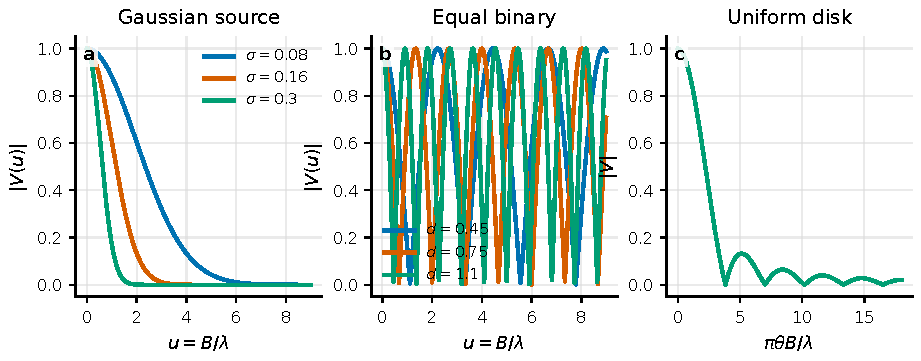
\includegraphics[width=0.9\linewidth]{figures/generated/chapter_01/ch01_fourier_visibility.pdf}
\caption{The normalized visibility \(|V|\) versus spatial frequency for several sky-brightness structures: a Gaussian source declines smoothly, equal-brightness binary stars produce cosine oscillations, and a uniform disk, because of its sharp edge, shows zeros and sidelobes. This is completely isomorphic to this chapter's temporal "spectral line shape \(\leftrightarrow\) fringe decay": the sinc sidelobes of a rectangular spectrum correspond to the Bessel sidelobes of a uniform disk; only the "frequency spectrum" is replaced by the "sky brightness distribution," and the "time delay" by the "spatial baseline."}
\label{fig:e09-fourier-visibility}
\end{figure}

This axis change is astonishingly powerful. The Wiener--Khinchin theorem says "\(g^{(1)}(\tau)\) is the Fourier transform of the power spectrum \(S(\nu)\)"; its spatial twin (the protagonist of the next chapter, the van Cittert--Zernike theorem) will say "\(\gamma_{12}\) is the Fourier transform of the sky brightness distribution \(I(l,m)\)." So every conclusion of this chapter has a spatial counterpart: the shape of the fringe decay tells us the spectral line shape, just as the shape of the visibility versus baseline tells us the \emph{source's angular structure}; the sinc sidelobes of a rectangular spectrum correspond to the Bessel sidelobes of a uniform disk (Fig.~\ref{fig:e09-fourier-visibility}); the coherence length \(\ell_c\) is to delay as some critical baseline is to angular scale. Shifting this whole intuition of temporal coherence over to space is our ticket into spatial coherence and imaging.

Carrying one sentence into the next chapter: \textbf{the visibility is the reading of first-order coherence, and first-order coherence gives the spectral line along the time axis and the image along the spatial baseline.} Chapter \ref{chap:e10} starts from \(\gamma_{12}\), uses the van Cittert--Zernike theorem to turn it into a Fourier component of the sky, and then uses intensity interferometry to measure \(|\gamma_{12}|^2\), stepping toward stellar angular diameters and imaging.

\section{Chapter Summary}
\label{sec:e09-summary}

\begin{itemize}
  \item \textbf{The fringe formula.} A two-path optical-path difference \(\Delta\) introduces the carrier phase \(\delta=2\pi\Delta/\lambda\) and time delay \(\tau=\Delta/c\), and the detected intensity is \(I(\delta)=I_1+I_2+2\sqrt{I_1I_2}\,|g^{(1)}(\tau)|\cos(\delta-\varphi(\tau))\), where \(\varphi(\tau)\) is the slow residual phase after removing the carrier (zero for a symmetric spectral line). The amplitude of the cosine term is proportional to the first-order degree of coherence \(|g^{(1)}|\).
  \item \textbf{The visibility is the reading of the degree of coherence.} \(\mathcal V=(I_{\max}-I_{\min})/(I_{\max}+I_{\min})=\dfrac{2\sqrt{I_1I_2}}{I_1+I_2}|g^{(1)}(\tau)|\); at equal intensity \(\mathcal V=|g^{(1)}(\tau)|\). The abstract "how much phase the field still remembers" becomes fringe contrast readable by eye.
  \item \textbf{Coherence length.} The fringes fade as the optical-path difference grows, with characteristic scale \(\ell_c=c\tau_c\simeq\lambda^2/\Delta\lambda\): about 1\,\(\mu\)m for white light, about 0.3\,mm for a 1\,nm narrowband, about 300\,m for a MHz laser.
  \item \textbf{The Wiener--Khinchin bridge.} \(g^{(1)}(\tau)\) is the Fourier transform of the normalized power spectrum; a rectangular spectrum gives \(|g^{(1)}|=|{\rm sinc}(\Delta\nu\tau)|\) (with zeros and sidelobes), a Lorentzian gives \(|g^{(1)}|=e^{-|\tau|/\tau_c}\) (pure exponential). Hence measuring the fringe decay with delay can infer the spectral line shape: the principle of Fourier-transform spectroscopy.
  \item \textbf{Two routes.} Amplitude interferometry directly measures the complex visibility (with phase) but requires the optical path stable to a fraction of a wavelength and is sensitive to atmospheric piston; intensity interferometry measures only \(|\mathcal V|^2\), losing phase, but needs only electronic alignment to a fraction of the response time (see the comparison table, leading into Chapter \ref{chap:e10}).
  \item \textbf{Change of axis to space.} Replace the time-delay version \(g^{(1)}(\tau)\) with the two-point spatial version \(\gamma_{12}\), with visibility \(\mathcal V=|\gamma_{12}|\); it is the protagonist of the next chapter's van Cittert--Zernike theorem and intensity interferometry.
\end{itemize}

\medskip
\noindent\textbf{Questions to Ponder.}
\begin{enumerate}
  \item A Michelson interferometer under white light shows colored fringes only when the two arms are almost equal in length; with a \(\Delta\lambda=1\,{\rm nm}\) narrowband filter, to how large does the allowed two-arm optical-path difference expand? Estimate using Eq.~\eqref{eq:e09-coherence-length}.
  \item The two path intensities are in the ratio \(I_1:I_2=4:1\); even if the light is fully coherent (\(|g^{(1)}|=1\)), what is the highest fringe visibility attainable? This shows that "not seeing full-amplitude fringes" need not mean incoherence.
  \item If the measured visibility decays as a pure exponential with delay, \(\mathcal V(\tau)=e^{-|\tau|/\tau_c}\), with \(\tau_c=1\,{\rm ns}\), what shape is the corresponding spectral line, and what is the linewidth \(\Delta\nu\)? Converted to wavelength, how "narrow" is this line?
\end{enumerate}
